\documentclass{beamer}

\usepackage[utf8x]{inputenc}
\usepackage{default}
\usepackage{subfigure}
\usepackage{listings}
%\usepackage[bars]{beamerthemetree} % Beamer theme v 2.2
\usetheme{Boadilla}
% Beamer theme v 3.0
\usecolortheme{seahorse}
% Beamer color theme

\AtBeginSection[]
{
   \begin{frame}
       \frametitle{Outline}
       \tableofcontents[currentsection]
   \end{frame}
}

\AtBeginSubsection[]
{
   \begin{frame}
       \frametitle{Outline}
       \tableofcontents[currentsection,currentsubsection]
   \end{frame}
}



\begin{document}


\title{MASON Retirement Age}
\author{Ernesto Carrella}
\date{May 2 2011}
\institute[George Mason University]{RA}


\frame{\titlepage}


\section{Introduction}

\frame{
\frametitle{The two souls of the paper}

\begin{itemize}
\item An experiment in replication
\pause
\item An experiment in MASON
\end{itemize}
}

\frame{
\frametitle{Replication}

\begin{itemize}
\item If we choose a very simple model, can we achieve ``numerical identity''?
\pause
\item No
\pause
\item Numerical identity is really hard
\end{itemize}


}

\frame{
\frametitle{MASON}

\begin{itemize}
\item \textit{Models are completely independent from visualization, which can be added, removed, or changed at any time}
\pause
\item Can we believe advertisement?
\pause
\item Maybe.
\end{itemize}


}

\section{Replication}

\frame{
\frametitle{The Good}
\begin{figure}
\centering
  \subfigure[Original Paper]{
   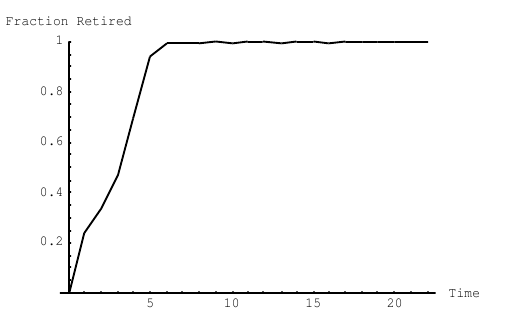
\includegraphics[scale =.40] {figs/figure4.png}
 }
 \subfigure[MASON replication]{
   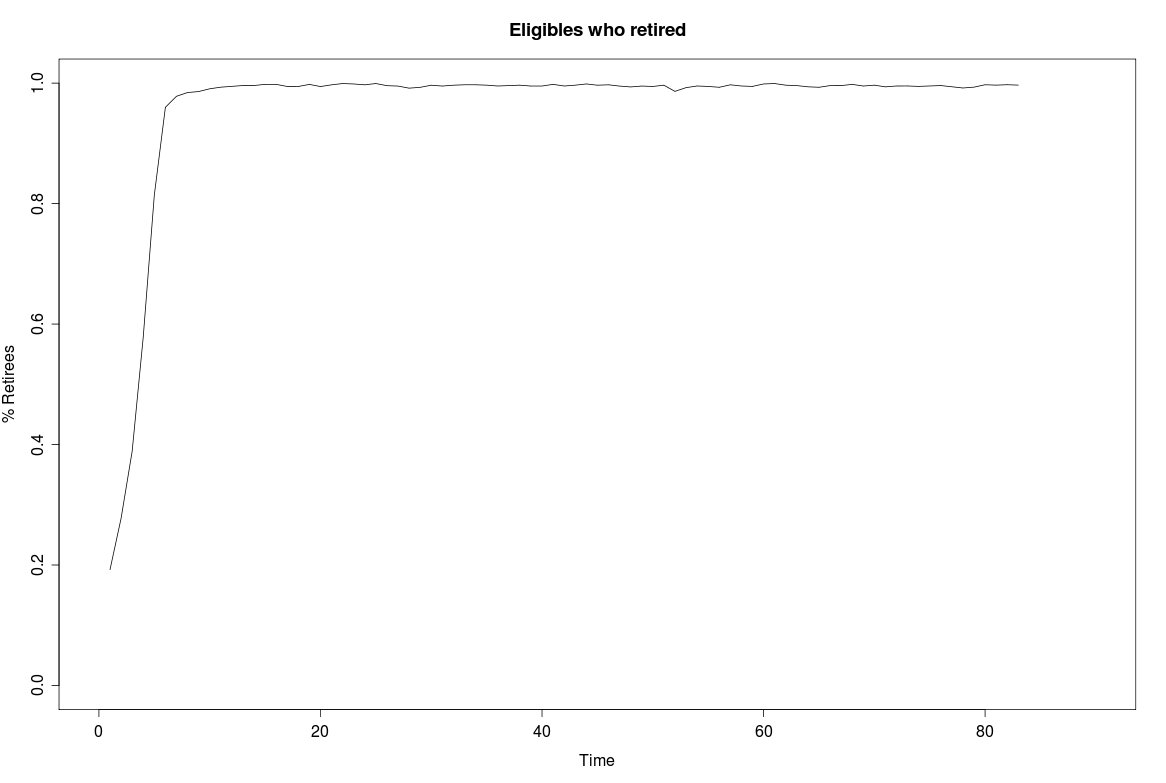
\includegraphics[scale =.13] {figs/figure4_replication.png}
 }

\caption{20\% rational agents case comparison}
\label{figure4}
\end{figure}


}

\frame{
\frametitle{The Good}
\begin{figure}
\centering
  \subfigure[Original Paper]{
   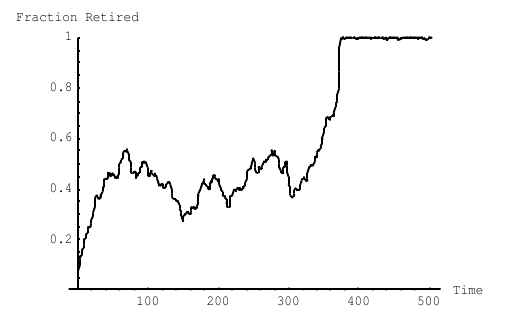
\includegraphics[scale =.40] {figs/figure5.png}
 }
 \subfigure[MASON replication]{
   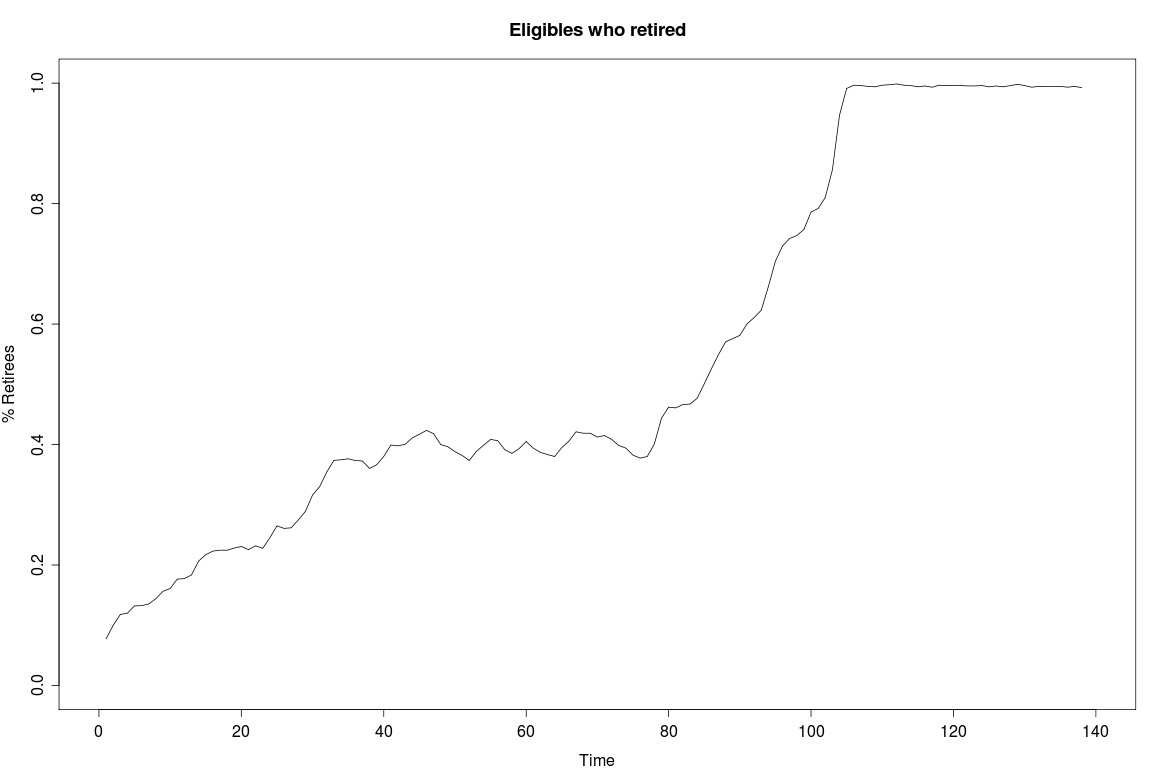
\includegraphics[scale =.13] {figs/figure5_replication.png}
 }

\caption{5\% rational agents case comparison}
\label{figure5}
\end{figure}

}

\frame{
\frametitle{The (kind of) good}

\begin{figure}
\centering
  \subfigure[Original Paper]{
   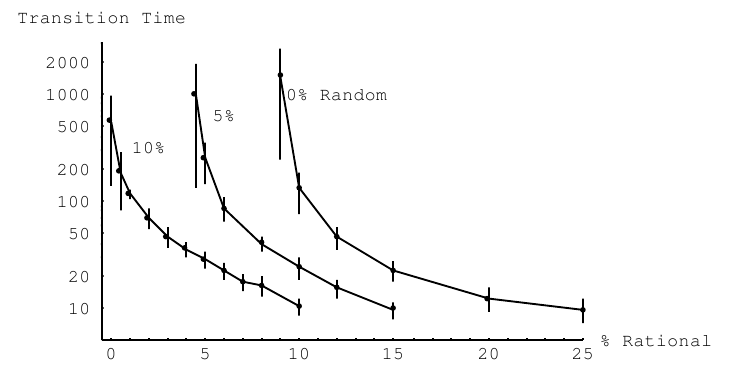
\includegraphics[scale =.35] {figs/figure6.png}
 }
 \subfigure[MASON replication]{
   \includegraphics[scale =.13] {figs/figure6_replication2.png}
 }

\caption{Rational agents sweep, black: 0\% random, red: 5\% random, blue 10\% random}
\label{figure6}
\end{figure}

}

\frame{
\frametitle{The (kind of) good}

\begin{figure}
\centering
  \subfigure[Original Paper]{
   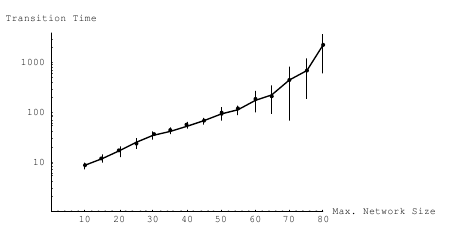
\includegraphics[scale =.40] {figs/figure8.png}
 }
 \subfigure[MASON replication]{
   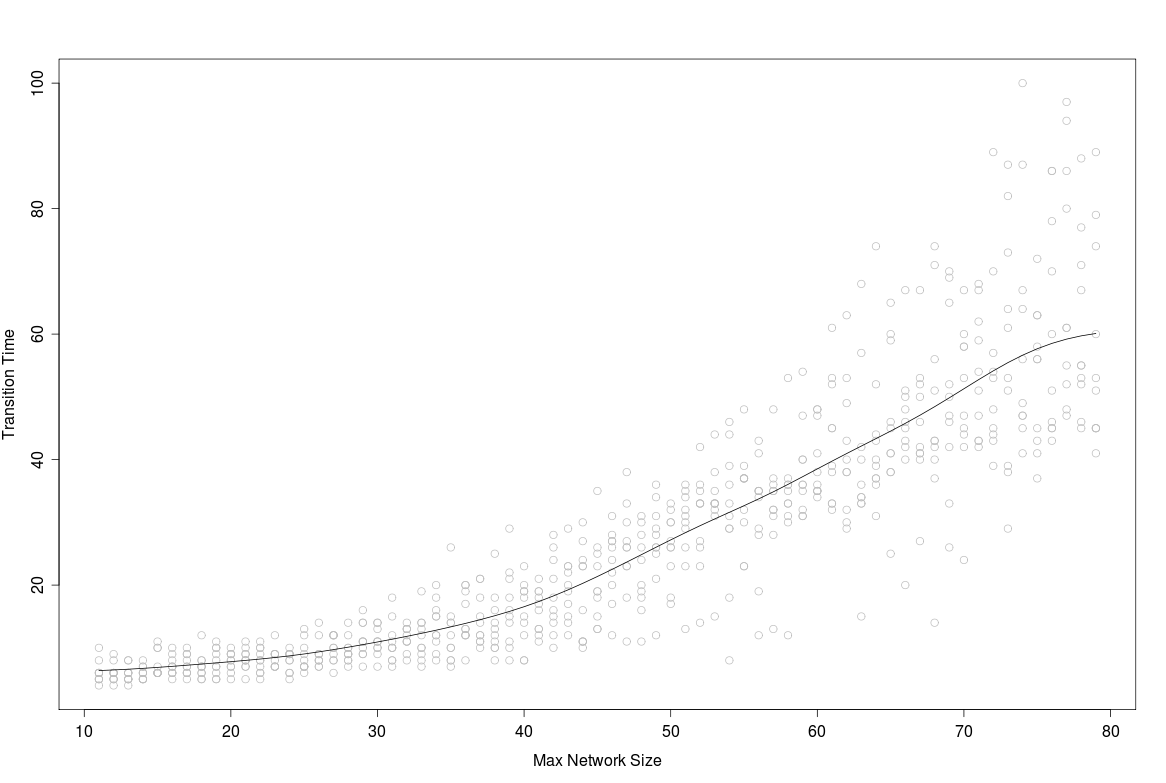
\includegraphics[scale =.13] {figs/figure8_replication.png}
 }

\caption{Changes in time to get full-retirement equilibrium by changing maximum network size. Grey dots represent runs}
\label{figure8}
\end{figure}

}


\frame{
\frametitle{The really bad}

\begin{figure}
\centering
   \includegraphics[scale =.25] {figs/failure.png}

\caption{Weird dynamics}
\label{figure8}
\end{figure}

}

\frame{
\frametitle{The weird}

\begin{figure}
 \begin{center}
  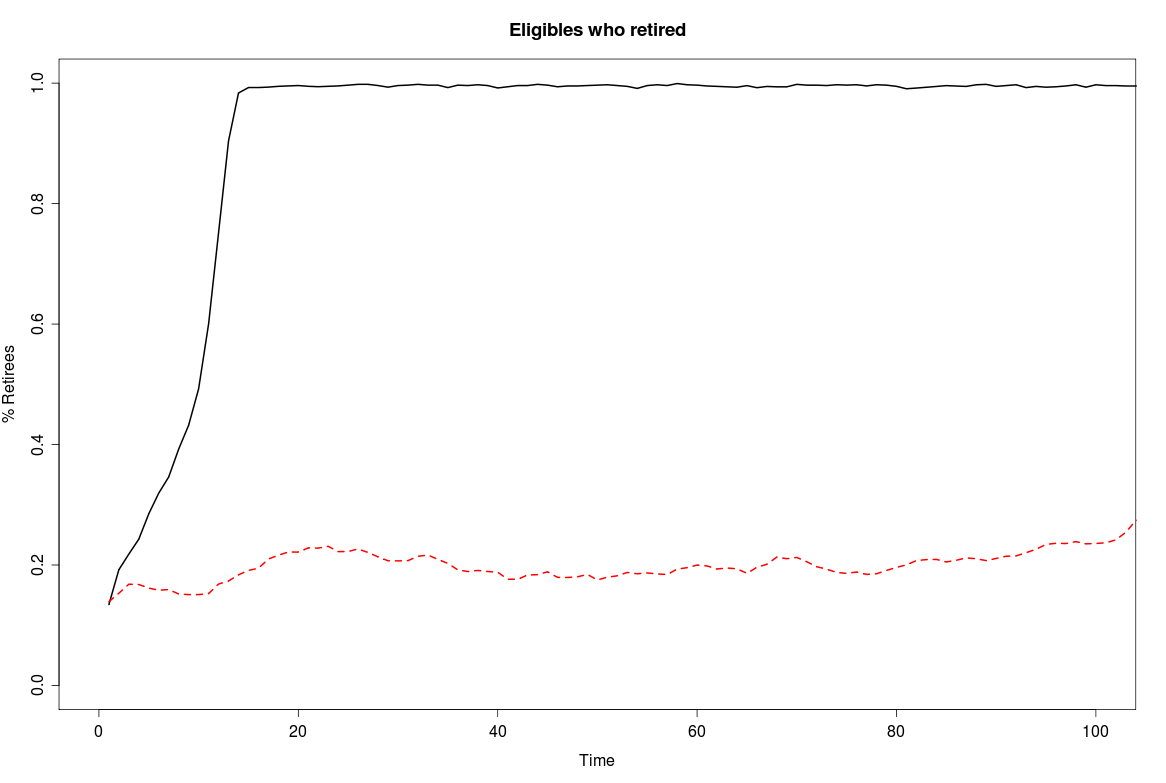
\includegraphics[scale=.20]{figs/laxstrict.png}
\caption{The black line is the simulation with strict threshold, the red line is without}
\label{laxstrict}
 \end{center}
\end{figure}
}

\section{Object Oriented Programming}

\frame{
\frametitle{The Advantages of Java}
\begin{itemize}
 \item Can use premade data structures
 \item Can use premade modelling structures
 \item Object-oriented programming!
\end{itemize}


}

\frame{
\frametitle{Amateur Perspective}

\begin{itemize}
 \item Never write twice
\pause
\item Small meaningful functions
\pause
\item Implementation Hiding
\pause
... sort of
\end{itemize}

}

\frame{
\frametitle{Agent Type}

\begin{itemize}
 \item Three types of agents
\pause
\begin{itemize}
\item Rational
\pause
\item Random
\pause
\item Imitator
\pause
\end{itemize}
\item Keep them as a class
\pause
\item Instantiate them in proportion
\end{itemize}

}


\frame{
\frametitle{It's UML Time!}

\begin{figure}
 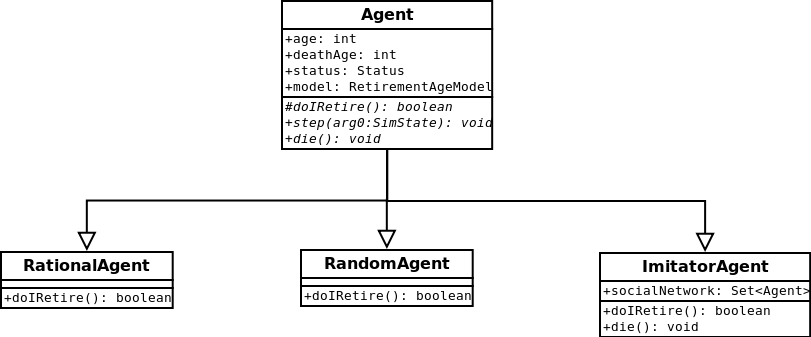
\includegraphics[scale=.3]{UML.png}
\end{figure}


}




\begin{frame}[fragile]
 \frametitle{Agent}

\begin{itemize}
 \item Interface vs Abstract Class
\pause
\end{itemize}

\begin{lstlisting}
	public void step(SimState arg0) {

		age++;

		if(age >= deathAge)
			this.die();

		else if (status == Status.WORKING)	
			status = doIRetire();	
	}
\end{lstlisting}



\end{frame}


\frame{
\frametitle{Overriding}


\begin{itemize}
 \item The difference in agents is only in the method \textit{doIRetire()}
\pause
 \item ImitatorAgent extends \textit{die() }
\pause
 \item All we need to do is schedule them.
\end{itemize}


}


\section{The Joy of Garbage Collection}

\frame{
\frametitle{The Garbage Collector}

\begin{itemize}
 \item It ``automatically'' destroys unused objects
\pause
 \item Automatically: unlinked objects
\pause
 \item Cannot be done manually
\end{itemize}

}

\frame{
\frametitle{Delete agents}

\begin{itemize}
 \item Do we really need to destroy them?
\pause
\includegraphics[scale=.20]{figs/monitor.png}
\pause
 \item Yes
\pause
 \item What links to them?
\pause
\begin{itemize}
 \item Simstate's table containing them
\pause
 \item and that's it?
\end{itemize}

\end{itemize}

}

\frame{
\frametitle{Schedule and Scheduling}

\begin{itemize}
 \item We schedule each agent separately
\pause
\item \textit{Schedule.scheduleRepeating()}
\pause
\item How does schedule works?
\pause
\item Heap
\end{itemize}


}

\frame{
\frametitle{How to remove a repeating steppable from the heap }

\begin{itemize}
\item Make the array steppable instead
\pause
\item Use Stoppable
\pause
\item \textit{\textbf{public} Stoppable scheduleRepeating(Steppable agent)}

\end{itemize}

}

\frame{
\frametitle{Delete agents 2}

\begin{itemize}
 \item Do we really need to destroy them?
\includegraphics[scale=.20]{figs/monitor.png}
 \item Yes
 \item What links to them?
\begin{itemize}
 \item Simstate's table containing them
 \item Schedule
\pause
 \item and that's it?
\end{itemize}

\end{itemize}

}

\frame{
\frametitle{Social Network }

\begin{itemize}
\item A set of Agents
\pause
\item These are references to your friends
\pause
\item As long as one of your friend is alive (or a friend of that friend...) you will not be recycled
\pause
\item This created enormous slowdowns, even after fixing for the other two
\pause
\item Morale: Garbage collector thinks you are smarter than you are

\end{itemize}

}



\end{document}